\documentclass[11pt,a4paper]{article}

% ============================================================
%  PACKAGES
% ============================================================
\usepackage[margin=2cm]{geometry}
\usepackage{tcolorbox}
\usepackage{amsmath,amssymb}
\usepackage{booktabs}
\usepackage{enumitem}
\usepackage{hyperref}
\usepackage{xcolor}
\usepackage{listings}
\usepackage{adjustbox}
\usepackage{tikz}
\usepackage{array}
\usepackage{multirow}

\usetikzlibrary{automata, positioning, arrows.meta}
\tcbuselibrary{breakable,skins}

% ============================================================
%  CUSTOM COMMANDS
% ============================================================
\newcommand{\fitmath}[1]{\begin{adjustbox}{max width=\linewidth}$\displaystyle #1$\end{adjustbox}}
\newcommand{\keytakeaway}[1]{%
  \par\vspace{0.3em}%
  \colorbox{yellow!60}{\parbox{\dimexpr\linewidth-2\fboxsep}{#1}}%
  \vspace{0.3em}}
\newcommand{\blank}{\sqcup}

% ============================================================
%  BOX DEFINITIONS
% ============================================================
\newtcolorbox{definitionbox}[1]{
  colback=blue!5, colframe=blue!60!black,
  fonttitle=\bfseries, title=#1, breakable, enhanced jigsaw
}

\newtcolorbox{conceptbox}[1]{
  colback=red!5, colframe=red!60!black,
  fonttitle=\bfseries, title=#1, breakable, enhanced jigsaw
}

\newtcolorbox{examplebox}[1]{
  colback=green!5, colframe=green!60!black,
  fonttitle=\bfseries, title=#1, breakable, enhanced jigsaw
}

\newtcolorbox{notebox}[1]{
  colback=orange!5, colframe=orange!60!black,
  fonttitle=\bfseries, title=#1, breakable, enhanced jigsaw
}

\newtcolorbox{templatebox}[1]{
  colback=violet!5, colframe=violet!60!black,
  fonttitle=\bfseries, title=#1, breakable, enhanced jigsaw
}

% ============================================================
%  LISTINGS CONFIG
% ============================================================
\lstset{
  basicstyle=\ttfamily\small,
  breaklines=true,
  breakatwhitespace=false,
  postbreak=\mbox{\textcolor{gray}{$\hookrightarrow$}\space},
  columns=fullflexible,
  keepspaces=true,
  xleftmargin=0pt,
  xrightmargin=0pt,
  frame=none,
  commentstyle=\color{gray},
}

% TikZ style
\tikzset{
    ->,
    >=Stealth,
    node distance=2.5cm,
    every state/.style={
        thick,
        fill=blue!5,
        minimum size=1cm
    },
    accepting/.style={double, double distance=1.5pt},
}

\title{\Huge\textbf{Algorithms \& Computability}\\[0.5em]
\LARGE How to Actually Solve the Exercises\\[0.3em]
\large A Skills Guide for Tutorials 1--4}
\author{AC Exercise Method Guide}
\date{Spring 2026}

\begin{document}
\maketitle
\tableofcontents
\newpage

% ============================================================
%  SECTION 0: THE REAL PROBLEM
% ============================================================
\section{The Real Problem (Read This First)}

\begin{conceptbox}{Why You Can Understand the Lectures But Can't Solve the Exercises}

\textbf{The Core Problem:} Understanding ``what a Turing machine is'' and being able to \emph{write formal answers about Turing machines} are two completely different skills. The lectures teach you concepts. The exercises test whether you can \textbf{operate with formal definitions} --- cite them precisely, construct machines from them, and build arguments using them as building blocks.

\textbf{Analogy:} Imagine you understand how chess pieces move. You can explain ``the bishop moves diagonally.'' But when someone puts a position in front of you and says ``find checkmate in 3 moves'' --- you freeze. You \emph{understand} chess, but you haven't practiced \emph{playing} chess. The exercises are the game. This guide teaches you the moves.

\textbf{What this guide does:}
\begin{itemize}
    \item Identifies the \textbf{9 exercise types} that appear in Tutorials 1--4
    \item For each type, gives you a \textbf{step-by-step template} you can follow
    \item Shows you \textbf{what a correct answer looks like} and what the grader expects
    \item Does NOT give you solutions --- it teaches you the \textbf{method} to find solutions yourself
\end{itemize}

\keytakeaway{The exercises are not testing whether you're smart. They're testing whether you can follow a formal recipe. This guide gives you the recipes.}
\end{conceptbox}

\subsection{The 9 Exercise Types (Map)}

Every exercise in Tutorials 1--4 falls into one of these categories:

\begin{center}
\renewcommand{\arraystretch}{1.4}
\begin{tabular}{c|l|l}
\toprule
\textbf{Type} & \textbf{Name} & \textbf{Where It Appears} \\
\midrule
1 & Definition Checking & T1-Ex1, T1-Ex2, T2-Ex3, T3-Ex1 \\
2 & Mechanical Tracing (Runs) & T1-Ex3, T1-Ex4 runs, T1-Ex5 runs \\
3 & DTM/NTM Construction & T1-Ex4, T1-Ex5, T2-Ex4, T3-Ex3 \\
4 & Simulation / Robustness & T2-Ex1, T2-Ex2 \\
5 & Spot the Error & T3-Ex2 \\
6 & Closure Properties & T2-Ex5, T3-Ex5 \\
7 & Computability Classification & T4-Ex1, T4-Ex2 \\
8 & Reduction Proofs & T4-Ex5 \\
9 & CE vs Computable Arguments & T3-Ex4, T4-Ex3, T4-Ex4 \\
\bottomrule
\end{tabular}
\end{center}

\subsection{What You Must Know Cold (Before Anything Else)}

\begin{conceptbox}{The 5 Definitions You Must Be Able to Write From Memory}

Before you can solve \emph{any} exercise, you need to be able to write these 5 things from memory on a blank sheet of paper. Not ``roughly know'' --- \textbf{write them out exactly}. If you can't, nothing else in this guide will help.

\begin{enumerate}
    \item \textbf{DTM definition:} $M = (Q, \Sigma, \Gamma, s, t, r, \delta)$ with $\delta : (Q \setminus \{t,r\}) \times \Gamma \to Q \times \Gamma \times \{-1, +1\}$

    Breaking it down:
    \begin{itemize}
        \item $Q$ = finite set of states
        \item $\Sigma$ = input alphabet (the symbols that can appear in the input)
        \item $\Gamma$ = tape alphabet (always $\Sigma \subset \Gamma$ and $\blank \in \Gamma$ but $\blank \notin \Sigma$)
        \item $s \in Q$ = start state
        \item $t \in Q$ = accept state
        \item $r \in Q$ = reject state, $t \neq r$
        \item $\delta$ = transition function: takes (current state, current symbol) and outputs (new state, symbol to write, direction to move)
        \item $\delta$ is only defined for states that are NOT $t$ or $r$ (the machine stops in those)
    \end{itemize}

    \item \textbf{Configuration:} $[q, \tau, \ell]$ where $q$ = state, $\tau$ = tape content (function $\mathbb{N} \to \Gamma$), $\ell$ = head position. Simplified notation: $[q, \text{tape contents}\ldots, \ell]$.

    \item \textbf{Computable language:} $L$ is computable $\iff$ there exists a \underline{halting} DTM $M$ such that $L(M) = L$. (Halting = M stops on \emph{every} input, both in $L$ and not in $L$.)

    \item \textbf{Computably-enumerable (CE) language:} $L$ is CE $\iff$ there exists a DTM $M$ (not necessarily halting) such that $L(M) = L$. (If $w \in L$, $M$ accepts. If $w \notin L$, $M$ may reject OR loop forever.)

    \item \textbf{NTM:} Same as DTM but $\delta : (Q \setminus \{t,r\}) \times \Gamma \to \mathcal{P}(Q \times \Gamma \times \{-1, +1\})$ (returns a \emph{set} of possible transitions). Accepts if \emph{at least one} computation path reaches $t$.
\end{enumerate}

\keytakeaway{Quiz yourself right now: cover the definitions above and try to write them on paper. If you can't, re-read them 3 times, then try again. This is prerequisite \#0.}
\end{conceptbox}

% ============================================================
%  TYPE 1: DEFINITION CHECKING
% ============================================================
\newpage
\section{Type 1: Definition Checking}

\begin{notebox}{What This Type Looks Like}
\textbf{Pattern:} You're given a statement (``Can a DTM do X?'' or ``Is this definition of CE correct?'') and you must say yes/no with justification.

\textbf{Where it appears:} T1-Ex1, T1-Ex2, T2-Ex3, T3-Ex1

\textbf{Analogy:} Think of it like a lawyer reading a contract. The question is: ``Does the contract allow this?'' You don't give your opinion --- you point to the specific clause (definition) that says yes or no. The answer is ALWAYS in the definition.
\end{notebox}

\subsection{The Method (Step by Step)}

\begin{templatebox}{Template: Definition Checking}
\begin{enumerate}
    \item \textbf{Write down the relevant formal definition} on your scratch paper. Not from memory of ``what it means'' --- write the actual mathematical definition with all its symbols.

    \item \textbf{Identify which part of the definition the question targets.} Is it about $\delta$? About $\Gamma$ vs $\Sigma$? About halting vs non-halting?

    \item \textbf{Answer by pointing to the definition.} Your answer should literally say: ``Yes/No, because the definition states that [quote the relevant part].''

    \item \textbf{If the question asks about a claim (true/false):} Try to either prove it (using the definition) or find a counterexample. Counterexamples are usually simpler.
\end{enumerate}
\end{templatebox}

\subsection{Worked Example: ``Can a DTM write the blank symbol?''}

\begin{examplebox}{Walking Through T1-Ex1.1}

\textbf{Question:} Can a DTM ever write the blank symbol $\blank$ on its tape?

\textbf{Step 1: Write down the relevant definition.}\\
The transition function has type:
\fitmath{\delta : (Q \setminus \{t,r\}) \times \Gamma \to Q \times \Gamma \times \{-1, +1\}}

The output includes $Q \times \textcolor{red}{\Gamma} \times \{-1,+1\}$. The second component is what gets \emph{written} to the tape.

\textbf{Step 2: Which part matters?}\\
The question asks about writing $\blank$. The written symbol comes from $\Gamma$ (the tape alphabet).

\textbf{Step 3: Answer by citing the definition.}\\
Yes, a DTM can write $\blank$, because $\blank \in \Gamma$ (by definition, the blank symbol is always in the tape alphabet), and $\delta$ outputs an element of $\Gamma$ as the symbol to write.

\keytakeaway{Notice: the answer is just ``look at the type signature of $\delta$, see that $\blank \in \Gamma$, done.'' No creativity needed.}
\end{examplebox}

\subsection{Worked Example: ``Is this definition of CE correct?''}

\begin{examplebox}{Walking Through T1-Ex2 (Checking Formal Statements)}

\textbf{Question:} ``A language $L$ is computably-enumerable if \underline{the language} halts in the state $t$ whenever $w \in L$.'' Correct or wrong?

\textbf{Step 1: Write down the correct definition.}\\
$L$ is CE if there exists a DTM $M$ such that $M$, given input $w$, halts in $t$ if $w \in L$ (and may not halt if $w \notin L$).

\textbf{Step 2: Compare word by word.}
\begin{itemize}
    \item The given statement says ``\textbf{the language} halts'' --- but \emph{languages don't halt}. Only \emph{Turing machines} halt. A language is just a set of strings.
    \item The given statement also doesn't say ``there exists a DTM $M$'' --- it's missing the quantifier.
\end{itemize}

\textbf{Step 3: Write the answer.}\\
WRONG: ``the language halts'' is nonsensical --- a language is a set of strings, it cannot halt. Turing machines halt, not languages. Also, the definition requires ``there exists a DTM $M$ such that...''

\keytakeaway{The trick for these: read EVERY word of the given statement and check it against the definition. The errors are usually: wrong subject (``language'' instead of ``DTM''), wrong quantifier (``every'' instead of ``exists''), or missing pieces.}
\end{examplebox}

\subsection{The Checklist for Definition-Checking Questions}

\begin{conceptbox}{Common Traps to Watch For}
When checking if a statement about CE/computable/NTM is correct, these are the things that are usually wrong:

\begin{center}
\renewcommand{\arraystretch}{1.3}
\begin{tabular}{l|l}
\toprule
\textbf{Trap} & \textbf{What's Wrong} \\
\midrule
``The language halts/accepts/rejects'' & Languages don't do things, DTMs do \\
``Every DTM $M$...'' & Should be ``there exists a DTM $M$'' \\
``If and only if $w \in L$'' for CE & CE only requires ``if'', not ``only if'' \\
``More than one computation'' for NTM & NTM needs ``at least one'', not ``more than one'' \\
``Every computation accepts'' for NTM & NTM needs ``at least one'', not ``every'' \\
``$M$ rejects or does not halt, then do X'' & You \emph{cannot detect} non-halting \\
``$M$ is a member of $L$'' & $L$ contains strings, not machines \\
\bottomrule
\end{tabular}
\end{center}

\keytakeaway{90\% of these questions test whether you confuse ``for all'' with ``there exists'' or whether you apply predicates to the wrong objects.}
\end{conceptbox}

\subsection{Counterexample Strategy (for True/False Claims)}

\begin{templatebox}{Template: Disproving a Claim}
When a question says ``Is this claim true? If not, give a counterexample'' (like T3-Ex1):

\begin{enumerate}
    \item \textbf{First instinct check:} Does the claim feel too strong? ``Every subset of a computable language is computable'' --- that would mean computability is ``inherited'' by all subsets, which would be very powerful.

    \item \textbf{Try the extreme case:} What's the biggest/simplest language you know?
    \begin{itemize}
        \item $\Sigma^*$ is computable (accept everything)
        \item $\emptyset$ is computable (reject everything)
        \item Every language $L$ is a subset of $\Sigma^*$
    \end{itemize}

    \item \textbf{Use a known non-computable language:} If the claim says ``every subset of $L$ is computable'', try $L = \Sigma^*$ and pick any non-computable $L' \subseteq \Sigma^*$ (like HP). Since HP $\subseteq \Sigma^*$ and HP is not computable, the claim is false.

    \item \textbf{Write the counterexample clearly:}
    \begin{itemize}
        \item ``Let $L = \Sigma^*$. This is computable (accepted by a DTM that always accepts).''
        \item ``Let $L' = \text{HP}$. Then $L' \subseteq L$ (every language is a subset of $\Sigma^*$).''
        \item ``But HP is not computable (proven in lecture). Contradiction.''
    \end{itemize}
\end{enumerate}

\keytakeaway{When disproving: always try $\Sigma^*$ or $\emptyset$ as your base language first, then pick HP or AP as the counterexample subset. This works surprisingly often.}
\end{templatebox}

% ============================================================
%  TYPE 2: MECHANICAL TRACING
% ============================================================
\newpage
\section{Type 2: Mechanical Tracing (Runs)}

\begin{notebox}{What This Type Looks Like}
\textbf{Pattern:} Given a DTM (as a $\delta$ table) and an input word, write out the complete run step by step.

\textbf{Where it appears:} T1-Ex3, T1-Ex4 (parts 3--5), T1-Ex5 (parts 2--4)

\textbf{Analogy:} This is like being a human debugger. You have the source code ($\delta$ table), the input, and you just step through it line by line. No thinking --- just table lookup. If you can read a table, you can do this.
\end{notebox}

\subsection{The Method (Step by Step)}

\begin{templatebox}{Template: Tracing a DTM Run}
\textbf{Setup:} You have $M = (Q, \Sigma, \Gamma, s, t, r, \delta)$ given as a table, and input $w = a_1 a_2 \ldots a_n$.

\begin{enumerate}
    \item \textbf{Write the initial configuration:} $[s, a_1 a_2 \ldots a_n \blank \ldots, 1]$
    \begin{itemize}
        \item State = $s$ (always start in $s$)
        \item Tape = the input followed by blanks
        \item Head position = 1 (leftmost cell)
    \end{itemize}

    \item \textbf{For each step, do exactly this:}
    \begin{enumerate}[label=(\alph*)]
        \item Look at current state $q$ and current symbol (the symbol at position $\ell$ on the tape)
        \item Find the row $q$ and column for that symbol in the $\delta$ table
        \item Read off $(q', b, d)$ from the table
        \item Write the new configuration: state becomes $q'$, the symbol at position $\ell$ on the tape changes to $b$, head moves to position $\ell + d$
        \item \textbf{Special case:} if head is at position 1 and $d = -1$, the head stays at position 1 (can't go left of the tape)
    \end{enumerate}

    \item \textbf{Stop when} the state is $t$ (accepted) or $r$ (rejected).

    \item \textbf{Write the full run using $\vdash_M$ notation:}\\
    $[\text{config}_0] \vdash_M [\text{config}_1] \vdash_M [\text{config}_2] \vdash_M \ldots \vdash_M [\text{final config}]$
\end{enumerate}
\end{templatebox}

\subsection{Worked Example: A Full Trace}

\begin{examplebox}{Tracing the DTM from T1-Ex3 on Input $aab$}

\textbf{Given $\delta$:}
\begin{center}
\begin{tabular}{c|c|c|c}
$\delta$ & $a$ & $b$ & $\blank$ \\
\hline
$s$ & $(h, \blank, +1)$ & $(r, b, +1)$ & $(t, \blank, +1)$ \\
$h$ & $(h, a, +1)$ & $(h, b, +1)$ & $(e, \blank, -1)$ \\
$e$ & $(r, a, +1)$ & $(g, \blank, -1)$ & $(r, \blank, +1)$ \\
$g$ & $(g, a, -1)$ & $(g, b, -1)$ & $(s, \blank, +1)$ \\
\end{tabular}
\end{center}

\textbf{Input:} $w = aab$

\textbf{Step-by-step:}

\begin{enumerate}
    \item \textbf{Config 0:} $[s, aab\blank\ldots, 1]$\\
    State = $s$, symbol at position 1 = $a$.\\
    Look up $\delta(s, a) = (h, \blank, +1)$.\\
    $\Rightarrow$ State becomes $h$, write $\blank$ at position 1, head moves to position 2.

    \item \textbf{Config 1:} $[h, \blank ab\blank\ldots, 2]$\\
    State = $h$, symbol at position 2 = $a$.\\
    Look up $\delta(h, a) = (h, a, +1)$.\\
    $\Rightarrow$ State stays $h$, write $a$ at position 2 (unchanged), head moves to 3.

    \item \textbf{Config 2:} $[h, \blank ab\blank\ldots, 3]$\\
    State = $h$, symbol at position 3 = $b$.\\
    Look up $\delta(h, b) = (h, b, +1)$.\\
    $\Rightarrow$ State stays $h$, write $b$ at position 3 (unchanged), head moves to 4.

    \item \textbf{Config 3:} $[h, \blank ab\blank\ldots, 4]$\\
    State = $h$, symbol at position 4 = $\blank$.\\
    Look up $\delta(h, \blank) = (e, \blank, -1)$.\\
    $\Rightarrow$ State becomes $e$, write $\blank$ (unchanged), head moves back to 3.

    \item \textbf{Config 4:} $[e, \blank ab\blank\ldots, 3]$\\
    State = $e$, symbol at position 3 = $b$.\\
    Look up $\delta(e, b) = (g, \blank, -1)$.\\
    $\Rightarrow$ State becomes $g$, write $\blank$ at position 3, head moves to 2.

    \item \textbf{Config 5:} $[g, \blank a\blank\blank\ldots, 2]$\\
    State = $g$, symbol at position 2 = $a$.\\
    Look up $\delta(g, a) = (g, a, -1)$.\\
    $\Rightarrow$ State stays $g$, write $a$ (unchanged), head moves to 1.

    \item \textbf{Config 6:} $[g, \blank a\blank\blank\ldots, 1]$\\
    State = $g$, symbol at position 1 = $\blank$.\\
    Look up $\delta(g, \blank) = (s, \blank, +1)$.\\
    $\Rightarrow$ State becomes $s$, head moves to 2.

    \item \textbf{Config 7:} $[s, \blank a\blank\blank\ldots, 2]$\\
    State = $s$, symbol at position 2 = $a$.\\
    Look up $\delta(s, a) = (h, \blank, +1)$.\\
    $\Rightarrow$ State becomes $h$, write $\blank$ at position 2, head moves to 3.

    \item \textbf{Config 8:} $[h, \blank\blank\blank\blank\ldots, 3]$\\
    State = $h$, symbol at position 3 = $\blank$.\\
    Look up $\delta(h, \blank) = (e, \blank, -1)$.\\
    $\Rightarrow$ State becomes $e$, head moves to 2.

    \item \textbf{Config 9:} $[e, \blank\blank\blank\blank\ldots, 2]$\\
    State = $e$, symbol at position 2 = $\blank$.\\
    Look up $\delta(e, \blank) = (r, \blank, +1)$.\\
    $\Rightarrow$ State becomes $r$. \textbf{STOP --- $r$ is the reject state.}
\end{enumerate}

\textbf{Final answer in compact notation:}
\fitmath{[s, aab\blank\ldots, 1] \vdash_M [h, \blank ab\blank\ldots, 2] \vdash_M [h, \blank ab\blank\ldots, 3] \vdash_M [h, \blank ab\blank\ldots, 4] \vdash_M [e, \blank ab\blank\ldots, 3] \vdash_M}
\fitmath{[g, \blank a\blank\ldots, 2] \vdash_M [g, \blank a\blank\ldots, 1] \vdash_M [s, \blank a\blank\ldots, 2] \vdash_M [h, \blank\blank\ldots, 3] \vdash_M [e, \blank\blank\ldots, 2] \vdash_M [r, \blank\blank\ldots, 3]}

\textbf{Result:} $aab$ is \textbf{rejected} by $M$.

\keytakeaway{This is pure mechanical bookkeeping. No thinking, just: look up (state, symbol) in table $\to$ write new config. If you can do one step, you can do all of them.}
\end{examplebox}

\subsection{Common Mistakes in Tracing}

\begin{conceptbox}{Things That Go Wrong When Tracing}
\begin{enumerate}
    \item \textbf{Forgetting to update the tape.} When $\delta$ says write $b$, the tape \emph{changes}. In the next step, you read the \emph{new} symbol, not the old one.

    \item \textbf{Wrong head position.} $+1$ means the head moves \emph{right} (position increases). $-1$ means it moves \emph{left} (position decreases). Don't mix them up.

    \item \textbf{Forgetting the left-boundary special case.} If head is at position 1 and direction is $-1$, the head \emph{stays} at position 1. This is the only case where the head doesn't move.

    \item \textbf{Reading the wrong column.} Double-check which symbol is at the current position. After the tape has been modified, the symbol might be different from the original input.
\end{enumerate}

\keytakeaway{Use your finger (or pen) to physically track the head position on your paper. Draw the tape if it helps. The most common mistake is losing track of where the head is.}
\end{conceptbox}

% ============================================================
%  TYPE 3: DTM/NTM CONSTRUCTION
% ============================================================
\newpage
\section{Type 3: DTM/NTM Construction}

\begin{notebox}{What This Type Looks Like}
\textbf{Pattern:} Given a language description, build a Turing machine that accepts it.

\textbf{Where it appears:} T1-Ex4, T1-Ex5, T2-Ex4, T3-Ex3

\textbf{Analogy:} This is like being an architect. Someone says ``I want a house with 3 bedrooms and a garage.'' You don't just start placing bricks --- you first sketch a floor plan (algorithm in words), then draw blueprints (states and transitions), then build (write the $\delta$ table). The exercises expect all three phases.
\end{notebox}

\subsection{The Method (Step by Step)}

\begin{templatebox}{Template: Constructing a DTM}
\begin{enumerate}
    \item \textbf{Phase 1: Understand the language}
    \begin{enumerate}[label=(\alph*)]
        \item Write out the language formally: $L = \{w \in \Sigma^* \mid \ldots\}$
        \item List 3--4 examples of words IN the language
        \item List 3--4 examples of words NOT in the language
        \item \textbf{Corner cases!} What about: the empty word $\varepsilon$? Single-character words? What if the input has unexpected symbols?
    \end{enumerate}

    \item \textbf{Phase 2: Algorithm in plain English}
    \begin{enumerate}[label=(\alph*)]
        \item Describe what a human would do to check if a word is in the language
        \item Use bullet points: ``First, look at the first letter. Then, scan right until...''
        \item Identify: what information do you need to \emph{remember} while scanning? Each piece of remembered info = a state (or set of states)
    \end{enumerate}

    \item \textbf{Phase 3: Translate to states}
    \begin{enumerate}[label=(\alph*)]
        \item Each ``mode'' or ``phase'' of the algorithm becomes a state
        \item Each ``thing to remember'' doubles the states (one state for ``remembering 0'', one for ``remembering 1'')
        \item ``Scan right past everything'' = a self-loop on all input symbols
        \item ``Stop when you see X'' = a transition on X that goes to a new state
    \end{enumerate}

    \item \textbf{Phase 4: Write the formal definition}
    \begin{enumerate}[label=(\alph*)]
        \item List $Q, \Sigma, \Gamma, s, t, r$
        \item Write the $\delta$ table
        \item \textbf{Fill every cell} --- even unreachable ones (put anything, e.g., $(r, \text{symbol}, +1)$)
    \end{enumerate}

    \item \textbf{Phase 5: Verify}
    \begin{enumerate}[label=(\alph*)]
        \item Trace the machine on your example words (both in $L$ and not in $L$)
        \item Trace on the corner cases
        \item Check: does it halt on ALL inputs? (If it should be a halting DTM)
    \end{enumerate}
\end{enumerate}
\end{templatebox}

\subsection{The Key Insight: States = Memory}

\begin{conceptbox}{How to Choose Your States}

\textbf{The fundamental principle:} A Turing machine's states are its memory. The tape head can only see ONE cell at a time. If the algorithm needs to ``remember'' something it saw earlier, that information must be encoded in the current state.

\textbf{Analogy:} You're walking through a dark tunnel with a flashlight (the head). You can only see one tile at a time. If you need to remember the color of the first tile while checking the last tile, you have to carry that information in your head (= in the state).

\textbf{Translation rules:}
\begin{center}
\renewcommand{\arraystretch}{1.3}
\begin{tabular}{l|l}
\toprule
\textbf{Algorithm says...} & \textbf{States become...} \\
\midrule
``Remember which letter the first symbol was'' & $q_0, q_1$ (one per possible letter) \\
``Scan right until blank'' & One state with self-loops on all non-blank symbols \\
``Go back to the start'' & One state with self-loops moving left \\
``Check if last letter matches remembered letter'' & $\text{check}_0, \text{check}_1$ (one per remembered letter) \\
``Mark this cell as visited'' & Write a special symbol (like $X$) on the tape \\
\bottomrule
\end{tabular}
\end{center}

\keytakeaway{States = what you remember. Tape modifications = what you write down as notes. Head movement = walking through the input.}
\end{conceptbox}

\subsection{Worked Example: First Letter = Last Letter}

\begin{examplebox}{Walking Through T1-Ex4 (Full Construction)}

\textbf{Language:} Words over $\{0,1\}$ whose first letter equals their last letter.

\textbf{Phase 1: Understand the language.}
\begin{itemize}
    \item IN the language: $0$, $1$, $00$, $11$, $010$, $101$, $0110$
    \item NOT in the language: $01$, $10$, $011$, $100$, $\varepsilon$
    \item Corner cases: $\varepsilon$ (no first/last letter $\Rightarrow$ reject), single chars like $0$ or $1$ (first = last $\Rightarrow$ accept)
\end{itemize}

\textbf{Phase 2: Algorithm in words.}
\begin{enumerate}
    \item Read the first letter and \emph{remember it}.
    \item If there's no first letter (tape is blank), reject.
    \item Scan right until you reach the end of the input (first $\blank$).
    \item Go one step left --- you're now on the last letter.
    \item Compare the last letter to the remembered first letter.
    \item If they match, accept. Otherwise, reject.
\end{enumerate}

\textbf{Phase 3: Translate to states.}
\begin{itemize}
    \item $s$: start state. Read first letter.
    \item $q_0$: ``I remember the first letter was 0.'' Scan right.
    \item $q_1$: ``I remember the first letter was 1.'' Scan right.
    \item $\text{check}_0$: ``I'm on the last letter and need it to be 0.''
    \item $\text{check}_1$: ``I'm on the last letter and need it to be 1.''
    \item $t$: accept. $r$: reject.
\end{itemize}

\textbf{Phase 4: Write the $\delta$ table.}
\begin{center}
\begin{tabular}{c|c|c|c}
$\delta$ & $0$ & $1$ & $\blank$ \\
\hline
$s$ & $(q_0, 0, +1)$ & $(q_1, 1, +1)$ & $(r, \blank, +1)$ \\
$q_0$ & $(q_0, 0, +1)$ & $(q_0, 1, +1)$ & $(\text{check}_0, \blank, -1)$ \\
$q_1$ & $(q_1, 0, +1)$ & $(q_1, 1, +1)$ & $(\text{check}_1, \blank, -1)$ \\
$\text{check}_0$ & $(t, 0, +1)$ & $(r, 1, +1)$ & $(r, \blank, +1)$ \\
$\text{check}_1$ & $(r, 0, +1)$ & $(t, 1, +1)$ & $(r, \blank, +1)$ \\
\end{tabular}
\end{center}

\textbf{Reading the table row by row:}
\begin{itemize}
    \item $s$: If first symbol is $0$, remember it (go to $q_0$). If $1$, remember it (go to $q_1$). If blank (empty input), reject.
    \item $q_0/q_1$: Scan right past all input symbols (self-loop). When we hit $\blank$, go left into the check state.
    \item $\text{check}_0$: We're on the last letter, and we need it to be $0$. If it is $0$, accept. If it's $1$, reject. If it's $\blank$ (this means the input was just one character and we're now left of it --- actually this handles the edge case where $\text{check}$ lands on blank, meaning reject).
\end{itemize}

\keytakeaway{The pattern ``remember something, scan to the end, compare'' covers a huge number of construction exercises. The structure is always: read $\to$ remember (via state) $\to$ scan (self-loop) $\to$ check.}
\end{examplebox}

\subsection{State Diagram Visualization}

\begin{examplebox}{What the Machine Looks Like as a Diagram}

\begin{center}
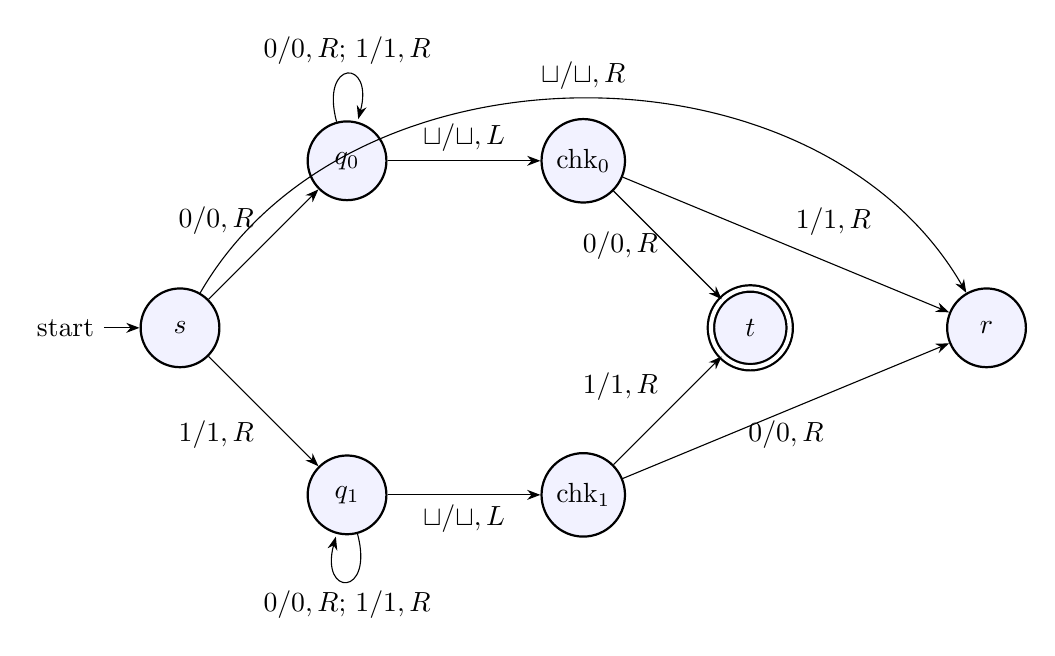
\begin{tikzpicture}[node distance=3cm, auto]
    \node[state, initial]   (s)    {$s$};
    \node[state]            (q0)   [above right of=s] {$q_0$};
    \node[state]            (q1)   [below right of=s] {$q_1$};
    \node[state]            (c0)   [right of=q0] {$\text{chk}_0$};
    \node[state]            (c1)   [right of=q1] {$\text{chk}_1$};
    \node[state, accepting] (t)    [below right of=c0] {$t$};
    \node[state]            (r)    [right of=t] {$r$};

    \path (s)  edge node {$0/0,R$} (q0)
          (s)  edge node[below left] {$1/1,R$} (q1)
          (s)  edge [bend left=60] node[above] {$\blank/\blank,R$} (r)
          (q0) edge [loop above] node {$0/0,R$; $1/1,R$} ()
          (q0) edge node {$\blank/\blank,L$} (c0)
          (q1) edge [loop below] node {$0/0,R$; $1/1,R$} ()
          (q1) edge node[below] {$\blank/\blank,L$} (c1)
          (c0) edge node[left] {$0/0,R$} (t)
          (c0) edge node {$1/1,R$} (r)
          (c1) edge node {$1/1,R$} (t)
          (c1) edge node[below] {$0/0,R$} (r);
\end{tikzpicture}
\end{center}

The self-loops on $q_0$ and $q_1$ are the ``scanning'' phase. The edges to $\text{chk}$ states are ``I reached the end.'' The edges from $\text{chk}$ to $t$ or $r$ are ``compare and decide.''
\end{examplebox}

\subsection{The Answer Format the Grader Expects}

\begin{conceptbox}{What to Actually Write on Your Exam Paper}

Based on the solutions, a DTM construction answer has \textbf{exactly these parts} in this order:

\begin{enumerate}
    \item \textbf{Formal language definition} (if asked): $L = \{a_1 a_2 \cdots a_n \mid a_j \in \{0,1\}, n \geq 1, a_1 = a_n\}$

    \item \textbf{Intuitive description} (2--4 bullet points): ``The DTM works as follows:''
    \begin{itemize}
        \item Store the first letter using states $q_0$ and $q_1$
        \item Scan right until blank
        \item Go left and compare
    \end{itemize}

    \item \textbf{Formal definition:} ``We define $M = (Q, \Sigma, \Gamma, s, t, r, \delta)$ with:''
    \begin{itemize}
        \item $Q = \{\ldots\}$
        \item $\Sigma = \{\ldots\}$
        \item $\Gamma = \{\ldots\}$
        \item $\delta$ given by the following table: $[\text{the table}]$
    \end{itemize}

    \item \textbf{Runs on example inputs} (if asked): Use the $\vdash_M$ notation.
\end{enumerate}

\keytakeaway{Always give the intuition BEFORE the formal definition. The grader wants to see that you understand what the machine does, not just that you can fill in a table.}
\end{conceptbox}

\subsection{NTM Construction: When and How}

\begin{conceptbox}{DTM vs NTM: When to Use Which}

\textbf{Use a DTM when:} The algorithm is deterministic --- at each step, there's only one thing to do. (T1-Ex4, T1-Ex5)

\textbf{Use an NTM when:} The problem requires \emph{guessing} something --- like where to split a string, or which nondeterministic branch to take. (T2-Ex4, T3-Ex3)

\textbf{The NTM trick:} Instead of trying all possibilities one by one, an NTM tries them all \emph{in parallel}. If any branch accepts, the whole machine accepts.

\textbf{Translation rule:}
\begin{itemize}
    \item ``Try all possible split points'' $\Rightarrow$ NTM: at each position, nondeterministically choose ``split here'' or ``continue''
    \item ``Guess two numbers'' $\Rightarrow$ NTM: nondeterministically write two numbers, then verify
    \item ``Check if infix XYZ exists'' $\Rightarrow$ NTM: nondeterministically guess where XYZ starts, then verify
\end{itemize}

\textbf{NTM $\delta$ table format:} Instead of $\delta(q,a) = (q', b, d)$, you write $\delta(q,a) = \{(q_1', b_1, d_1), (q_2', b_2, d_2)\}$ --- a \emph{set} of possible transitions.

\keytakeaway{NTM = ``guess and verify.'' The nondeterminism handles the guessing; after the guess, the verification is usually deterministic.}
\end{conceptbox}

% ============================================================
%  TYPE 4: SIMULATION / ROBUSTNESS
% ============================================================
\newpage
\section{Type 4: Simulation / Robustness Proofs}

\begin{notebox}{What This Type Looks Like}
\textbf{Pattern:} ``Show that variant X of DTMs can be simulated by standard DTMs.'' Or equivalently: ``Show that adding feature X doesn't make DTMs more powerful.''

\textbf{Where it appears:} T2-Ex1 (stay direction), T2-Ex2 (doubly-infinite tape)

\textbf{Analogy:} Someone claims their fancy new car (DTM variant) can reach places that a normal car can't. You need to show that a normal car can reach all the same places --- maybe by taking a slightly different route, but it gets there.
\end{notebox}

\subsection{The Method}

\begin{templatebox}{Template: Simulation Proof}
\begin{enumerate}
    \item \textbf{Identify the difference:} What can the variant do that a standard DTM can't? (e.g., ``stay in place'' or ``move left past cell 1'')

    \item \textbf{Show how to fake it:} How can a standard DTM achieve the same effect using only its standard operations?
    \begin{itemize}
        \item ``Stay'' = go right then go left (2 steps instead of 0, but same result)
        \item ``Doubly-infinite tape'' = shift content when hitting the left boundary
    \end{itemize}

    \item \textbf{Construct $M'$ formally:}
    \begin{itemize}
        \item $M' = (Q', \Sigma, \Gamma', s, t, r, \delta')$ --- same $\Sigma$, $s$, $t$, $r$
        \item $Q' = Q \cup \{\text{auxiliary states}\}$ --- add new states for the workaround
        \item $\delta'$ = copy of $\delta$ for normal transitions, plus new transitions for the workaround
    \end{itemize}

    \item \textbf{State the correctness claim:}\\
    ``$M'$ outcome-simulates $M$: if $M$ halts/accepts on input $w$, then $M'$ halts/accepts on input $w$.''

    \item \textbf{Argue why it's correct} (usually obvious from the construction, but say it explicitly).
\end{enumerate}
\end{templatebox}

\subsection{Worked Example: The ``Stay'' Direction}

\begin{examplebox}{How to Simulate ``Stay'' (T2-Ex1)}

\textbf{The difference:} The variant allows $\delta(q,a) = (q', b, 0)$ --- don't move the head.

\textbf{How to fake it with a standard DTM:}\\
Go right one step, then go left one step. You end up at the same cell.

\textbf{New states needed:} For each state $q'$ that should be the target of a ``stay'' transition, add an auxiliary state $q'_L$ that means ``I need to go left to get back to where I was.''

\textbf{New transitions:}
\begin{itemize}
    \item If the original has $\delta(q, a) = (q', b, 0)$ (stay), replace with:
    \begin{itemize}
        \item $\delta'(q, a) = (q'_L, b, +1)$ --- write $b$, go right, remember we need to go back
        \item $\delta'(q'_L, c) = (q', c, -1)$ for all $c \in \Gamma$ --- whatever we see, leave it unchanged, go left, arrive at $q'$
    \end{itemize}
    \item If the original has $\delta(q, a) = (q', b, +1)$ or $(q', b, -1)$ (normal), copy unchanged: $\delta'(q, a) = \delta(q, a)$
\end{itemize}

\textbf{Why it's correct:} After the two moves (right then left), the head is back at the original position, in state $q'$, with symbol $b$ written --- exactly the same as the ``stay'' transition. The cell we visited in between is left unchanged.

\keytakeaway{The simulation pattern is: identify the ``exotic'' operation $\to$ replace it with a sequence of standard operations that achieves the same effect $\to$ add auxiliary states to manage the extra steps.}
\end{examplebox}

% ============================================================
%  TYPE 5: SPOT THE ERROR
% ============================================================
\newpage
\section{Type 5: Spot the Error in Proofs}

\begin{notebox}{What This Type Looks Like}
\textbf{Pattern:} Given a ``proof'' that's wrong, find the error and explain why.

\textbf{Where it appears:} T3-Ex2

\textbf{Analogy:} Think of it like proofreading a recipe. The recipe claims to make chocolate cake, but you know from experience that the recipe produces something else. Your job: find the step where they added salt instead of sugar.
\end{notebox}

\subsection{The Method}

\begin{templatebox}{Template: Spotting Errors in Proofs About CE/Computable}
The most common errors in proofs about CE languages:

\begin{enumerate}
    \item \textbf{The ``Simulate $M$ on $w$'' trap:} If $M$ doesn't halt on $w$, then the simulation \emph{never finishes}. So any code that says ``Simulate $M$ on $w$. If $M$ rejects, then do X'' --- the ``do X'' part is \emph{never reached} if $M$ loops. The proof implicitly assumes $M$ halts, but for CE languages, $M$ might not halt.

    \item \textbf{The ``detect non-halting'' trap:} A proof says ``If $M$ does not halt on $w$, then $M'$ accepts.'' This is nonsense --- there is no way for a DTM to detect that another DTM doesn't halt. That would solve the halting problem.

    \item \textbf{The ``swap accept/reject'' trap:} Swapping $t$ and $r$ for a CE language's DTM does NOT give you the complement. If $M$ loops on $w \notin L$, then swapping $t$ and $r$ still causes $M'$ to loop on $w \notin L$ --- so $M'$ doesn't accept $w$ either. You end up with $L(M') \neq \overline{L}$.
\end{enumerate}

\textbf{Detection strategy:} For each step in the ``proof,'' ask yourself:
\begin{itemize}
    \item Does this step assume $M$ halts? (If $M$ is only CE, it might not halt.)
    \item Does this step try to detect non-halting? (Impossible.)
    \item Try a \textbf{concrete counterexample}: pick a DTM $M$ that loops on some input and trace through the ``proof.''
\end{itemize}
\end{templatebox}

\begin{examplebox}{The Classic Counterexample for ``Swap t and r''}

\textbf{The flawed proof says:} ``Given CE language $L$ with DTM $M$, construct $M'$ that accepts when $M$ rejects and vice versa. Then $L(M') = \overline{L}$.''

\textbf{Counterexample:} Let $M$ be a DTM over $\Sigma = \{a\}$ where $\delta(s, a) = (s, a, +1)$ and $\delta(s, \blank) = (s, a, +1)$.

This machine \emph{never halts} on any input. So $L(M) = \emptyset$.

Now build $M'$ by swapping $t$ and $r$. But $M$ never reaches $t$ or $r$ --- it loops forever. So $M'$ also loops forever on every input. Therefore $L(M') = \emptyset$.

But $\overline{L} = \overline{\emptyset} = \Sigma^*$, and $L(M') = \emptyset \neq \Sigma^*$.

\keytakeaway{The swap trick fails because looping inputs remain looping. $M$ loops $\Rightarrow$ $M'$ loops (swapping $t$ and $r$ doesn't help if neither is ever reached).}
\end{examplebox}

% ============================================================
%  TYPE 6: CLOSURE PROPERTIES
% ============================================================
\newpage
\section{Type 6: Closure Properties}

\begin{notebox}{What This Type Looks Like}
\textbf{Pattern:} ``Prove that the class of computable/CE languages is closed under [union/intersection/concatenation/complement/...].''

\textbf{Where it appears:} T2-Ex5, T3-Ex5

\textbf{Analogy:} If you have two cookie cutters (DTMs for $L_1$ and $L_2$) and someone asks ``can you make a cookie that satisfies BOTH shapes?'' --- you need to show how to combine the two cutters into one that does the job.
\end{notebox}

\subsection{The Method}

\begin{templatebox}{Template: Closure Proof}
\begin{enumerate}
    \item \textbf{Start with:} ``Let $L_1$ and $L_2$ be [computable/CE] languages. By definition, there exist [halting] DTMs $M_1$ and $M_2$ such that $L(M_1) = L_1$ and $L(M_2) = L_2$.''

    \item \textbf{Construct $M$} that accepts the combined language ($L_1 \cup L_2$, $L_1 \cap L_2$, $L_1 \cdot L_2$, etc.):

    \begin{itemize}
        \item \textbf{Union:} ``On input $w$: Simulate $M_1$ on $w$. If it accepts, accept. Otherwise, simulate $M_2$ on $w$. If it accepts, accept. Otherwise, reject.'' (For CE: use parallel simulation --- run both step-by-step.)

        \item \textbf{Intersection:} ``On input $w$: Simulate $M_1$ on $w$. If it rejects, reject. Otherwise, simulate $M_2$ on $w$. Accept iff $M_2$ accepts.''

        \item \textbf{Complement:} ``On input $w$: Simulate $M_1$ on $w$. If it accepts, reject. If it rejects, accept.'' (\textbf{Only works for computable languages!} $M_1$ must halt.)

        \item \textbf{Concatenation:} Use NTM: ``Nondeterministically split $w = w_1 w_2$. Simulate $M_1$ on $w_1$ and $M_2$ on $w_2$. Accept if both accept.''
    \end{itemize}

    \item \textbf{Argue correctness:} ``$M$ accepts $w$ iff [both/either] $M_1$ and $M_2$ accept their inputs, which happens iff $w \in L_1 [\text{op}]\ L_2$.''

    \item \textbf{Argue halting} (if proving closure for computable languages): ``$M$ halts because $M_1$ halts (it's a halting DTM) and $M_2$ halts.''
\end{enumerate}
\end{templatebox}

\begin{conceptbox}{The Critical Difference: Computable vs CE Closure}

\textbf{Why complement closure fails for CE:}

For \textbf{computable} languages, $M$ is halting, so ``simulate $M$ and swap the answer'' works.

For \textbf{CE} languages, $M$ might loop. If $M$ loops, you can't ``swap'' --- you never get an answer to swap. That's why CE is NOT closed under complement.

\textbf{Why union needs special handling for CE:}

For \textbf{computable}: Run $M_1$, then $M_2$. Since both halt, this terminates.

For \textbf{CE}: If you run $M_1$ first and it loops, you never get to run $M_2$ --- even if $M_2$ would accept! \textbf{Fix: parallel simulation (dovetailing).} Run one step of $M_1$, one step of $M_2$, one step of $M_1$, one step of $M_2$, \ldots Accept as soon as either one accepts.

\keytakeaway{For computable: sequential simulation is fine (both halt). For CE: you often need parallel simulation (dovetailing) to avoid getting stuck in a loop.}
\end{conceptbox}

% ============================================================
%  TYPE 7: COMPUTABILITY CLASSIFICATION
% ============================================================
\newpage
\section{Type 7: Computability Classification}

\begin{notebox}{What This Type Looks Like}
\textbf{Pattern:} Given a language $L$, determine: is it computable, CE-but-not-computable, or not even CE? If computable, describe a halting DTM.

\textbf{Where it appears:} T4-Ex1, T4-Ex2

\textbf{Analogy:} Think of it like a border patrol officer. Someone hands you a passport (a language). You need to decide: ``Is this person allowed in (computable)?'' or ``They might be allowed but I can't tell for sure (CE)?'' or ``Definitely not allowed (not CE)?'' Your tool is: what can a DTM \emph{actually check} in finite time?
\end{notebox}

\subsection{The Decision Flowchart}

\begin{templatebox}{Template: Is $L$ Computable?}

Ask yourself these questions in order:

\begin{enumerate}
    \item \textbf{Is the property ``finite'' or ``bounded''?}
    \begin{itemize}
        \item ``$M$ has more than 5 states'' $\to$ just count the states in the encoding. \textbf{Computable.}
        \item ``$M$ accepts $w$ in less than 1000 steps'' $\to$ simulate for 1000 steps and check. \textbf{Computable.}
        \item Key insight: if you can put a \emph{fixed upper bound} on the computation you need to do, it's computable.
    \end{itemize}

    \item \textbf{Is it a syntactic property of the encoding?}
    \begin{itemize}
        \item Properties of the \emph{encoding} $\lceil M \rceil$ (number of states, alphabet size, specific transitions) can be checked by just parsing the string. \textbf{Computable.}
    \end{itemize}

    \item \textbf{Does it require running $M$ for an unbounded number of steps?}
    \begin{itemize}
        \item ``$M$ accepts $w$'' = ``$M$ accepts $w$ in a \textbf{finite} number of steps'' = AP. \textbf{Not computable.}
        \item ``$M$ halts on $w$'' = HP. \textbf{Not computable.}
        \item ``$L(M) \neq \emptyset$'' = NEP. \textbf{Not computable.}
    \end{itemize}

    \item \textbf{Is it a disguised version of a known problem?}
    \begin{itemize}
        \item ``$M$ accepts $w$ in a finite number of steps'' = ``$M$ accepts $w$'' = AP. The word ``finite'' is a red herring --- accepting \emph{always} takes finitely many steps.
        \item ``$M$ halts in accepting or rejecting state'' = ``$M$ halts'' = HP. A DTM can \emph{only} halt in $t$ or $r$, so this adds nothing.
    \end{itemize}
\end{enumerate}
\end{templatebox}

\begin{examplebox}{Worked Example: Classifying T4-Ex1 Languages}

\textbf{$L_1 = \{\langle \lceil M \rceil \rangle \mid M \text{ has more than 5 states}\}$}\\
Property of the encoding (syntactic). Just parse the encoding and count states.\\
$\Rightarrow$ \textbf{Computable.} DTM: check that the first 6 symbols of the encoding are all $1$'s.

\textbf{$L_2 = \{\langle \lceil M \rceil, w \rangle \mid M \text{ accepts } w \text{ in less than 1000 steps}\}$}\\
Bounded computation. Simulate $M$ on $w$ for exactly 1000 steps.\\
$\Rightarrow$ \textbf{Computable.} DTM: simulate for 1000 steps, accept if $M$ accepted during simulation, reject otherwise.

\textbf{$L_3 = \{\langle \lceil M \rceil, w \rangle \mid M \text{ accepts } w \text{ in a finite number of steps}\}$}\\
\textbf{Trap:} ``finite number of steps'' sounds bounded, but it's not. ``$M$ accepts $w$ in a finite number of steps'' is exactly the same as ``$M$ accepts $w$'' (because acceptance always takes finitely many steps). This is exactly AP.\\
$\Rightarrow$ \textbf{Not computable.}

\textbf{$L_4 = \{\langle \lceil M \rceil, w \rangle \mid M \text{ halts in } t \text{ or } r\}$}\\
\textbf{Trap:} A DTM can \emph{only} halt in $t$ or $r$ (those are the only halting states). So ``halts in $t$ or $r$'' is exactly ``halts.'' This is HP.\\
$\Rightarrow$ \textbf{Not computable.}

\keytakeaway{The key skill here is recognizing disguised versions of AP and HP. If it boils down to ``does $M$ accept $w$?'' or ``does $M$ halt on $w$?'' without a bound, it's not computable.}
\end{examplebox}

\subsection{Writing the DTM for Computable Cases}

\begin{templatebox}{Template: Describing a Halting DTM for a Computable Language}
The expected answer format:

\begin{enumerate}
    \item State that the language is computable.
    \item Describe the DTM: ``Consider the following halting DTM $M$:''
    \begin{itemize}
        \item ``On input $w$:''
        \item Step 1: Check if input has the right format (if it involves encodings)
        \item Step 2: Do the bounded check
        \item Step 3: Accept or reject based on the result
    \end{itemize}
    \item Argue that the DTM halts: ``This DTM halts because [the simulation is bounded / we only check a fixed number of symbols / etc.].''
\end{enumerate}

You do NOT need to give a full $\delta$ table for these. A clear algorithmic description is sufficient, as long as it's obvious that a DTM could implement it.
\end{templatebox}

% ============================================================
%  TYPE 8: REDUCTIONS
% ============================================================
\newpage
\section{Type 8: Reduction Proofs}

\begin{notebox}{What This Type Looks Like}
\textbf{Pattern:} ``Show that language $L$ is not computable by reducing from a known non-computable language.''

\textbf{Where it appears:} T4-Ex5

\textbf{Analogy:} You want to prove that Problem B is hard. You know Problem A is hard. So you show: ``If someone could solve B, they could also solve A --- but we know A can't be solved. Therefore B can't be solved either.'' It's a proof by contradiction using a translation.
\end{notebox}

\subsection{What a Reduction Actually Is}

\begin{definitionbox}{Many-One Reduction ($\leq_m$)}

\textbf{Plain English:}\\
A reduction from $A$ to $B$ is a computable function $f$ that translates every input for $A$ into an input for $B$, in a way that preserves the answer. If $x$ is a yes-instance of $A$, then $f(x)$ is a yes-instance of $B$. If $x$ is a no-instance of $A$, then $f(x)$ is a no-instance of $B$.

\textbf{Formal Definition:}
\fitmath{A \leq_m B \quad\text{if there exists a computable function } f : \Sigma^* \to \Sigma^* \text{ such that } x \in A \iff f(x) \in B}

\textbf{What it means:}
\begin{itemize}
    \item If $A \leq_m B$ and $A$ is not computable, then $B$ is not computable either.
    \item Intuition: $B$ is \emph{at least as hard} as $A$.
    \item Direction matters: you reduce FROM the known hard problem TO the new problem.
\end{itemize}
\end{definitionbox}

\subsection{The Method}

\begin{templatebox}{Template: Reduction Proof (``$L$ is not computable'')}
\begin{enumerate}
    \item \textbf{Choose your known non-computable language.} Usually AP (acceptance problem) or HP (halting problem).

    \item \textbf{Define the reduction function $f$.} Given an input to the known problem, construct an input to $L$.\\
    The most common pattern: given $\langle \lceil M \rceil, w \rangle$, construct a new DTM $\mathcal{E}_{M,w}$ whose behavior depends on whether $M$ accepts $w$.

    \item \textbf{The ``$\mathcal{E}_{M,w}$ construction'' (the master template):}
    \begin{itemize}
        \item Define a new DTM $\mathcal{E}_{M,w}$ that works as follows:
        \item ``On input $x$ (which $\mathcal{E}_{M,w}$ ignores):''
        \begin{enumerate}
            \item Erase $x$ from the tape.
            \item Write $w$ on the tape.
            \item Simulate $M$ on $w$.
            \item If $M$ accepts, then [do whatever makes $\mathcal{E}_{M,w}$ satisfy the target property].
        \end{enumerate}
        \item Key insight: $\mathcal{E}_{M,w}$ ignores its own input! Its behavior depends entirely on whether $M$ accepts $w$.
    \end{itemize}

    \item \textbf{Show the equivalence:}
    \begin{itemize}
        \item If $\langle \lceil M \rceil, w \rangle \in \text{AP}$, then $M$ accepts $w$, so $\mathcal{E}_{M,w}$ does [something], so $\lceil \mathcal{E}_{M,w} \rceil \in L$.
        \item If $\langle \lceil M \rceil, w \rangle \notin \text{AP}$, then $M$ doesn't accept $w$, so $\mathcal{E}_{M,w}$ doesn't do [something], so $\lceil \mathcal{E}_{M,w} \rceil \notin L$.
    \end{itemize}

    \item \textbf{Define $f$:}
    \fitmath{f(x) = \begin{cases} \lceil \mathcal{E}_{M,w} \rceil & \text{if } x = \langle \lceil M \rceil, w \rangle \\ \varepsilon & \text{otherwise} \end{cases}}

    \item \textbf{Conclude:} ``We have shown AP $\leq_m$ $L$. Since AP is not computable, $L$ is not computable either.''
\end{enumerate}
\end{templatebox}

\subsection{Worked Example: NEP is Not Computable}

\begin{examplebox}{Walking Through T4-Ex5}

\textbf{Goal:} Show that $\text{NEP} = \{\lceil M \rceil \mid L(M) \neq \emptyset\}$ is not computable.

\textbf{Step 1:} Reduce from AP $= \{\langle \lceil M \rceil, w \rangle \mid M \text{ accepts } w\}$.

\textbf{Step 2:} Given $\langle \lceil M \rceil, w \rangle$, define $\mathcal{E}_{M,w}$:

\begin{quote}
``On input $x$:
\begin{enumerate}
    \item Erase $x$ from the tape.
    \item Write $w$ on the tape.
    \item Simulate $M$ on $w$.
    \item If $M$ accepts $w$, then $\mathcal{E}_{M,w}$ accepts (if $M$ rejects, $\mathcal{E}_{M,w}$ rejects too).''
\end{enumerate}
\end{quote}

\textbf{Step 3: The key observation.}
\begin{itemize}
    \item $\mathcal{E}_{M,w}$ ignores its input $x$. It always simulates $M$ on $w$.
    \item If $M$ accepts $w$: then $\mathcal{E}_{M,w}$ accepts \emph{every} input $\Rightarrow$ $L(\mathcal{E}_{M,w}) = \Sigma^* \neq \emptyset$ $\Rightarrow$ $\lceil \mathcal{E}_{M,w} \rceil \in \text{NEP}$.
    \item If $M$ does not accept $w$: then $\mathcal{E}_{M,w}$ accepts \emph{no} input $\Rightarrow$ $L(\mathcal{E}_{M,w}) = \emptyset$ $\Rightarrow$ $\lceil \mathcal{E}_{M,w} \rceil \notin \text{NEP}$.
\end{itemize}

\textbf{Step 4:} Therefore:
\fitmath{\langle \lceil M \rceil, w \rangle \in \text{AP} \iff \lceil \mathcal{E}_{M,w} \rceil \in \text{NEP}}

Define $f(x) = \lceil \mathcal{E}_{M,w} \rceil$ if $x = \langle \lceil M \rceil, w \rangle$, and $f(x) = \varepsilon$ otherwise.

The function $f$ is computable (it just manipulates the encoding). So AP $\leq_m$ NEP. Since AP is not computable, NEP is not computable either.

\keytakeaway{The $\mathcal{E}_{M,w}$ trick works for many reductions: build a machine that ignores its own input and instead simulates $M$ on $w$. Then the target property of $\mathcal{E}_{M,w}$ depends entirely on whether $M$ accepts $w$.}
\end{examplebox}

% ============================================================
%  TYPE 9: CE vs COMPUTABLE
% ============================================================
\newpage
\section{Type 9: CE vs Computable Arguments}

\begin{notebox}{What This Type Looks Like}
\textbf{Pattern:} Show that a language is CE (but possibly not computable), or use the theorem ``$L$ is computable iff both $L$ and $\overline{L}$ are CE.''

\textbf{Where it appears:} T3-Ex4 (HP is CE), T4-Ex3 (the iff theorem), T4-Ex4 ($\overline{\text{AP}}$ is not CE)
\end{notebox}

\subsection{The Three Key Tools}

\begin{conceptbox}{The Three Tools for CE/Computable Arguments}

\textbf{Tool 1: ``Simulate and see what happens'' (showing something is CE).}\\
To show $L$ is CE, construct a DTM that accepts $w \in L$ (but may loop on $w \notin L$).\\
Template: ``On input $w$: Simulate [something]. If it accepts/halts, accept.''\\
The machine doesn't need to handle the non-membership case --- looping is fine for CE.

\textbf{Tool 2: The Complement Theorem.}\\
$L$ is computable $\iff$ both $L$ and $\overline{L}$ are CE.\\
\textbf{To prove $\Rightarrow$:} If $L$ is computable, then both $L$ and $\overline{L}$ have halting DTMs. Halting DTMs are special cases of DTMs, so both are CE.\\
\textbf{To prove $\Leftarrow$:} Run the DTM for $L$ and the DTM for $\overline{L}$ in parallel (dovetailing). One of them \emph{must} accept (since every $w$ is in either $L$ or $\overline{L}$). If the $L$-machine accepts first, accept. If the $\overline{L}$-machine accepts first, reject.

\textbf{Tool 3: Proof by contradiction (showing something is NOT CE).}\\
``Assume $\overline{L}$ is CE. Then both $L$ and $\overline{L}$ are CE. By Tool 2, $L$ is computable. But we know $L$ is not computable. Contradiction. So $\overline{L}$ is not CE.''
\end{conceptbox}

\subsection{Worked Example: HP is CE}

\begin{examplebox}{Walking Through T3-Ex4}

\textbf{Goal:} Show HP $= \{\langle \lceil M \rceil, w \rangle \mid M \text{ halts on } w\}$ is CE.

\textbf{Construct the DTM $\mathcal{H}$:}

``On input $x$:
\begin{enumerate}
    \item If $x$ is not of the form $\langle \lceil M \rceil, w \rangle$, reject.
    \item Otherwise, simulate $M$ on $w$.
    \item If $M$ halts (either accepts or rejects), then accept.''
\end{enumerate}

\textbf{Why this works:}
\begin{itemize}
    \item If $\langle \lceil M \rceil, w \rangle \in \text{HP}$ (i.e., $M$ halts on $w$): the simulation eventually halts, so $\mathcal{H}$ accepts. Good.
    \item If $\langle \lceil M \rceil, w \rangle \notin \text{HP}$ (i.e., $M$ doesn't halt on $w$): the simulation runs forever, so $\mathcal{H}$ doesn't halt. That's fine --- for CE, we only need to accept members, not reject non-members.
\end{itemize}

\keytakeaway{Showing something is CE is usually easy: just simulate and accept if the simulation terminates successfully. The hard part of CE problems is usually showing something is NOT CE (which requires the complement theorem or a reduction).}
\end{examplebox}

\subsection{Worked Example: $\overline{\text{AP}}$ is Not CE}

\begin{examplebox}{Walking Through T4-Ex4}

\textbf{Goal:} Show $\overline{\text{AP}}$ is not CE.

\textbf{Proof (3 lines):}
\begin{enumerate}
    \item Assume towards contradiction that $\overline{\text{AP}}$ is CE.
    \item We know AP is CE (proven in lecture/similar to HP being CE).
    \item Then both AP and $\overline{\text{AP}}$ are CE, so by the Complement Theorem, AP is computable.
    \item But we proved in lecture that AP is NOT computable. Contradiction.
    \item Therefore $\overline{\text{AP}}$ is not CE. \qed
\end{enumerate}

\keytakeaway{This proof pattern is extremely common: if you know $L$ is CE but not computable, then $\overline{L}$ cannot be CE (otherwise $L$ would be computable by the complement theorem).}
\end{examplebox}

% ============================================================
%  PUTTING IT ALL TOGETHER
% ============================================================
\newpage
\section{Putting It All Together: Your Study Plan}

\begin{conceptbox}{The Concrete Steps to Take}

\textbf{Phase 1: Definitions (30 minutes).}\\
Write out the 5 definitions from Section 1.3 on a blank piece of paper, from memory, 3 times. If you get stuck, look once, then try again. Don't move to Phase 2 until you can write all 5 without looking.

\textbf{Phase 2: Mechanical Tracing (45 minutes).}\\
Take the DTM from T1-Ex3 and trace it on inputs: $ab$, $ba$, $bb$, $a$, $\varepsilon$. Don't look at solutions. Just follow the $\delta$ table mechanically. This builds the ``muscle memory'' for the notation.

\textbf{Phase 3: One Construction (60 minutes).}\\
Pick a language you haven't seen before (make one up: ``words that start and end with 0'' or ``words with even length''). Follow the 5-phase template from Section 4. Write the full DTM. Trace it on 3 inputs to verify.

\textbf{Phase 4: One Proof (45 minutes).}\\
Try the closure proof for union: ``computable languages are closed under union.'' Follow the template from Section 7. Write it out in full.

\textbf{Phase 5: One Reduction (60 minutes).}\\
Try to show that $\text{TOTAL} = \{\lceil M \rceil \mid M \text{ halts on every input}\}$ is not computable. Use the reduction template from Section 9. (Hint: reduce from HP.)

\textbf{Total: about 4 hours.} After this, every exercise in Tutorials 1--4 should feel like a variation of something you've already done.
\end{conceptbox}

\subsection{Quick Reference: Which Template for Which Exercise}

\begin{center}
\renewcommand{\arraystretch}{1.4}
\begin{tabular}{l|l|l}
\toprule
\textbf{Exercise asks you to...} & \textbf{Use Type} & \textbf{Section} \\
\midrule
``Is this statement correct?'' & Definition Checking & \S2 \\
``Is this claim true/false?'' & Definition Checking + Counterexample & \S2.4 \\
``Give the run of $M$ on $w$'' & Mechanical Tracing & \S3 \\
``Construct a DTM for $L$'' & DTM Construction & \S4 \\
``Construct an NTM for $L$'' & NTM Construction & \S4.6 \\
``Show variant can be simulated'' & Simulation / Robustness & \S5 \\
``Find the error in this proof'' & Spot the Error & \S6 \\
``Show class closed under $X$'' & Closure Properties & \S7 \\
``Is $L$ computable?'' & Computability Classification & \S8 \\
``Show $L$ is not computable'' & Reduction & \S9 \\
``Show $L$ is (not) CE'' & CE vs Computable & \S10 \\
\bottomrule
\end{tabular}
\end{center}

\subsection{The Answer Format Cheat Sheet}

\begin{conceptbox}{How Long Should Your Answers Be?}

Based on the official solutions:

\begin{itemize}
    \item \textbf{Definition checking:} 2--3 sentences. State the answer, cite the definition, done.
    \item \textbf{Tracing:} Just write the chain of configurations. No explanation needed.
    \item \textbf{DTM construction:} Intuitive description (3--5 bullet points) + formal definition ($Q, \Sigma, \Gamma, \delta$ table) + runs on examples.
    \item \textbf{Simulation:} Intuitive idea (1 paragraph) + formal construction of $M'$ + correctness argument (1 paragraph).
    \item \textbf{Closure proof:} 1 paragraph setup + DTM description (numbered steps) + 1 paragraph arguing correctness and halting.
    \item \textbf{Reduction:} Construction of $\mathcal{E}_{M,w}$ + equivalence argument ($x \in A \iff f(x) \in B$) + conclusion.
    \item \textbf{CE argument:} Usually 3--5 lines total.
\end{itemize}

\keytakeaway{Most answers are shorter than you think. The solutions are precise and concise --- they don't ramble. Say exactly what needs to be said, cite the right definition or construction, and stop.}
\end{conceptbox}

\end{document}
